\documentclass[conference]{IEEEtran}
\usepackage{graphicx, multicol, latexsym, amsmath, amssymb}
\usepackage{blindtext}
\usepackage{subfigure}
\usepackage{caption}
%\usepackage{capt-of}
%\usepackage{tabu}
%\usepackage{hyperref}
%\usepackage{booktabs}% for better rules in the table
%\usepackage{anysize} % Soporte para el comando \marginsize
%\usepackage{adjustbox}
\usepackage{float}
\usepackage{wrapfig}
\ifCLASSINFOpdf
\else
\fi
\hyphenation{op-tical net-works semi-conduc-tor}
\begin{document}

\title{End-To-End Keyword Spotting}
\author{\IEEEauthorblockN{Stefano Ivancich}
\IEEEauthorblockA{Department of\\Information Engineering\\
University of Padova, Italy\\
Email: stefano.ivancich@studenti.unipd.it}
\and
\IEEEauthorblockN{Luca Masiero}
\IEEEauthorblockA{Department of\\Information Engineering\\
University of Padova, Italy\\
Email: luca.masiero.8@studenti.unipd.it}}

\maketitle

\begin{abstract}
In this paper, we present an end-to-end approach for the keyword spotting task, consisting of a sliding window of one second, a Voice Activity detection module, a feature extraction module, a neural network model and a fusion rule.

We explore the application of a 1D Convolutional Neural Network (CNN) that directly learns a representation from the audio signal, a Depth Wise Convolution (DSConv) and an ensemble of the best models.
The proposed models achieve a maximum accuracy of 96.6\% with a small footprint of 127K parameters on the Google Speech Commands dataset V2 (for the 10-commands and 21-commands recognition task).

We also compare the performances of those networks on different feature extraction methods such as 80 Mel, 40 MFCCs and 40MFCCs + deltas.
\end{abstract}

\IEEEpeerreviewmaketitle
\begin{IEEEkeywords}
Human voice, Command recognition, Deep learning, Keyword spotting.
\end{IEEEkeywords}

\section{Introduction}
The goal of keyword spotting is to detect a relatively small set of predefined keywords in a stream of user utterances, usually in the context of an intelligent agent on a mobile phone or a consumer “smart home” device. Such a capability complements fully automatic speech recognition, which is typically performed in the cloud. Since the cloud-based interpretation of speech input requires transferring audio recordings from the user’s device, significant privacy implications should be kept in mind. Therefore, on-device keyword spotting has two main objectives: the first one concerns the recognition of common commands such as “on” and “off” (as well as other frequent words such as “yes” and “no”): this recognition can be accomplished directly on the user’s device; secondly, keyword spotting can be used to detect “command triggers” such as “hey Siri”, which provides explicit cues for interactions directed at the device. It is additionally desirable that such models have a small footprint (for example, measured in the number of model parameters) so they can be deployed on low power and performance-limited devices.

In recent years, neural networks have been shown to provide effective solutions to the small-footprint keyword spotting problem. Research typically focuses on a trade-off between achieving a high detection accuracy, having, on the other hand, a small footprint. Compact models are usually variants derived from a full model that sacrifices accuracy for a smaller model footprint.

In this work, we focus on convolutional neural networks (CNNs), a class of models that has been successfully applied to small-footprint keyword spotting; in particular, we explore the use of Depthwise Separable Convolutions and 1D CNN.

In this paper we will: 
\begin{itemize}
\setlength{\itemsep}{0pt}
  \setlength{\parskip}{0pt}
  \setlength{\parsep}{0pt}
\item present an end-to-end architecture for the key-word-spotting task;
\item try different audio features (raw data, 80 Mels, 40 MFCC and 40 MFCC with deltas and delta-deltas);
\item train different type of neural networks (1D CNN on raw data and DSConv CNN on features);
\item build an ensemble of the best models;
\item compare prediction speed and the number of parameters between the models.
\end{itemize}

The report is structured as follows. In Section II we present the current state of the art in the speech recognition field, in Section III we show our approach in order to tackle the problem and in Section IV we explain the pre-processing techniques used. In Section V we describe the various architectures we used, in Section VI we report their results and in Section VII we make some extra considerations on future developments and improvements.

\hfill September 22, 2020
%\subsection{Subsection Heading Here}
%Subsection text here.
%\subsubsection{Subsubsection Heading Here}
%Subsubsection text here.

\section{Related work}
The first system similar to a modern ASR was built in the 1952 by researchers at Bell laboratories and was able to recognize numerical digits from speech using formants of the input audio. These formants are a concentration of the acoustic energy around a particular frequency in the input file wave. 
For the next thirty years, various researchers developed devices capable of recognize vowels and consonants using different types of features (like phonemes), until the introduction, in the mid 1980s, of the Hidden Markov Models (HMMs). This approach represented a significant shift from simple pattern recognition methods, based on templates and a spectral distance measure, to a statistical method for speech processing [LABINER] and was possible thank to the incredible advancements in the computer computational power during those years.
In recent times, however, the HMMs were challenged by the introduction of Deep Learning and several architectures that work very well with these type of problems: Convolutional Neural Networks take advantage of weight-sharing and the convolution operation (which is shift-invariant in the data representation domain), Recurrent Neural Networks (RNN) are able to store a great quantity of information.
Our two neural networks are inspired by [7] and [8]. 
In [7] the authors apply 1D CNN on raw signals for environment sound classification; we slightly modified the structure to adapt it to our task. In [8] the authors made some improvement on the MobileNet for Mobile Vision Applications using DSConv. 

\section{Processing Pipeline}
The aim of the end-to-end architecture we propose, represented in \textbf{\textit{Figure 1}}, is to handle audio signals of variable lengths and learn from the audio signal received.
\subsection{Variable Audio Length}
One of the main challenges of neural networks in audio processing is that the length of the input sample should be fixed but the sound captured may have various duration. For this reason, it is necessary to adapt the model making it able to deal with audio signals of different lengths. Moreover, a model must be used for continuous prediction of input audio signals. One way to avoid this constraint, imposed by the input layer of the neural network, is to split the audio signal into several frames of fixed length using a sliding window of one second width.

For long contiguous audio recordings, instead of increasing the input dimension of the network (and consequently increasing the number of parameters and its complexity), it is preferable to split the audio waveform into shorter frames: in this way, we keep the network compact so it can process audio waveforms of any length.

However, letting the model process each frame is too expensive ( from the computational point of view). For this reason, we can use a VAD (Voice Activity Detection) or a Silence Filter to let the model process just the frames containing voice. This component should be very compact, not so expensive and fast; it could be part of a software or even a little piece of hardware (like some home device that we use nowadays).
Only a batch of subsequent windows will be processed. For each of these windows a Feature Extraction module will extract 80 Mels, 40 MFCC, 40MFCC+deltas or no extraction at all: this will be the input of our model.

\subsection{Aggregation of Audio Frames}
During the classification we need to aggregate the predictions to come up to a decision, as illustrated in Figure 1; for this reason, different fusion rules can be used to reach a final decision, such as the \textit{majority vote} or the \textit{sum rule}.

\begin{figure*}
\centering
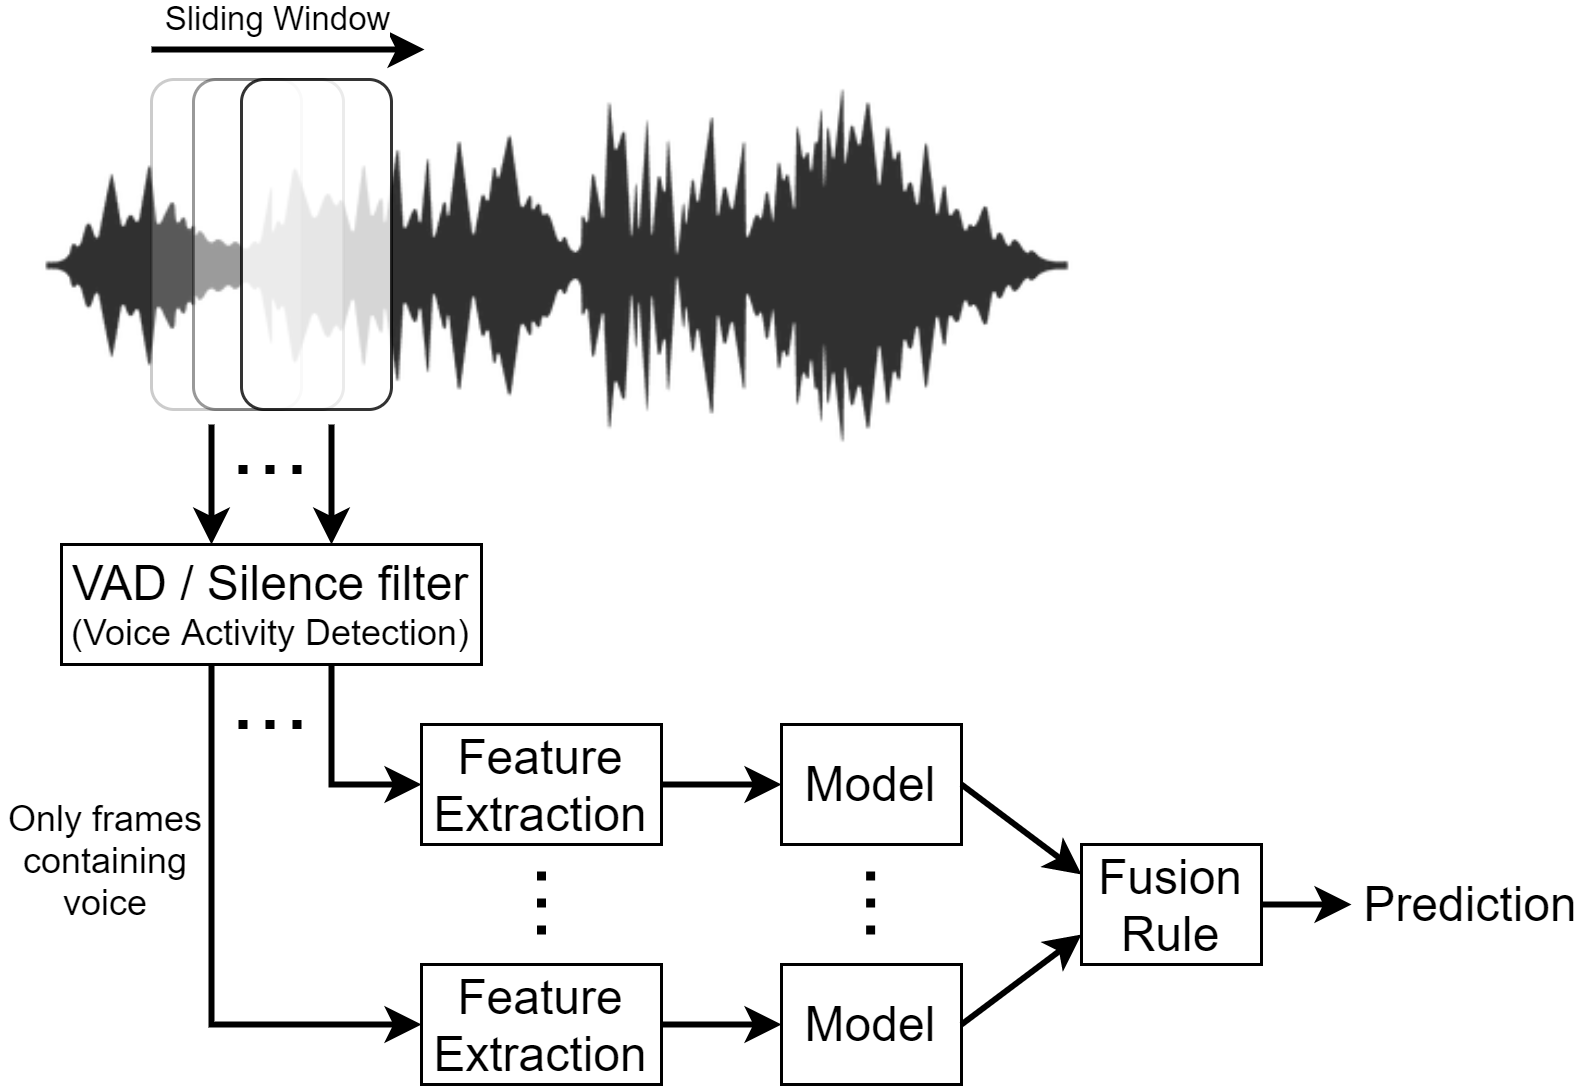
\includegraphics[scale=0.27]{End-To-End}

\begin{small}\textit{\textbf{Figure 1}: MANCA DESCRIZIONE}
\end{small}
\end{figure*}

\section{4.	Signals and Features}
As stated in Section I, we used the Google Speech Dataset V2. This dataset contains 105,829 audio files in .wav format (duration =  one second) divided in 30 classes, plus an additional class containing 5 different type of noise of variable duration (about 10 seconds for each file).

The core words are "Yes", "No", "Up", "Down", "Left", "Right", "On", "Off", "Stop", "Go", "Zero", "One", "Two", "Three", "Four", "Five", "Six", "Seven", "Eight", and "Nine". To help distinguish unrecognized words, there are also ten auxiliary words, which most speakers only said once: "Bed", "Bird", "Cat", "Dog", "Happy", "House", "Marvin", "Sheila", "Tree", and "Wow".

We decided to create two different datasets:
\begin{itemize}
\item the first one is made of ten classes ("Yes", "No", "Up", "Down", "Left", "Right", "On", "Off", "Stop", "Go"), where each class contains approximately 3,600 files;
\item the secondo is made of twenty-one classes ("Yes", "No", "Up", "Down", "Left", "Right", "On", "Off", "Stop", "Go", "Zero", "One", "Two", "Three", "Four", "Five", "Six", "Seven", "Eight", "Nine" and “Unknown”), where each class contains approximately 3,600 files, except for the “Unknown” class that contains all the remaining auxiliary words.
\end{itemize}

\subsection{Dataset Partitioning}
We divided both datasets into train-validation-test sets as suggested by Google into the dataset’s README file and we used a split of 30000-3000-3000 for the 10 classes dataset and 84000-9000-11000 for the twenty-one remaining classes. The training set is used to train the network, while the validation one is used to evaluate the network performance during the training and to allow early-stopping to save the model with the lowest validation error, preventing overfitting. The test set is used to evaluate the network’s final score with the best performance.

\subsection{Features extraction}
We decided to study four different types of features in order to compare them and tried to see which was the best able to solve our problem:
\begin{itemize}
\item \textbf{No feature extraction}: we trained a specific model (1D CNN) directly on the raw signal (a 16,000 elements vector);
\item \textbf{80 Mel spectrogram}: we took the Fourier Transform of (a windowed excerpt of) the raw signal and mapped the powers of the spectrum obtained into the mel scale (using triangular overlapping windows);
\item \textbf{40 Mel-frequency cepstral coefficients (MFCC)}: those coefficients are obtained after the computation of the Discrete Cosine Transform (DCT) on the logarithm of the Mel spectrogram;
\item \textbf{40 MFCC + Delta + Delta-Delta}: matrix containing the MFCCs previously computed, their first derivative (Delta) and second derivative (Delta-Delta).
\end{itemize}
We used the \textit{Librosa Python Library} to compute those features, in particular we used the following functions: \texttt{librosa.feature.melspectrogram(...), librosa.power\_to\_db(...), librosa.feature.mfcc(...), librosa.feature.delta(...)}.

\section{5.	Learning Framework}
\subsection{1D CNN on raw data}

\begin{figure*}
\centering
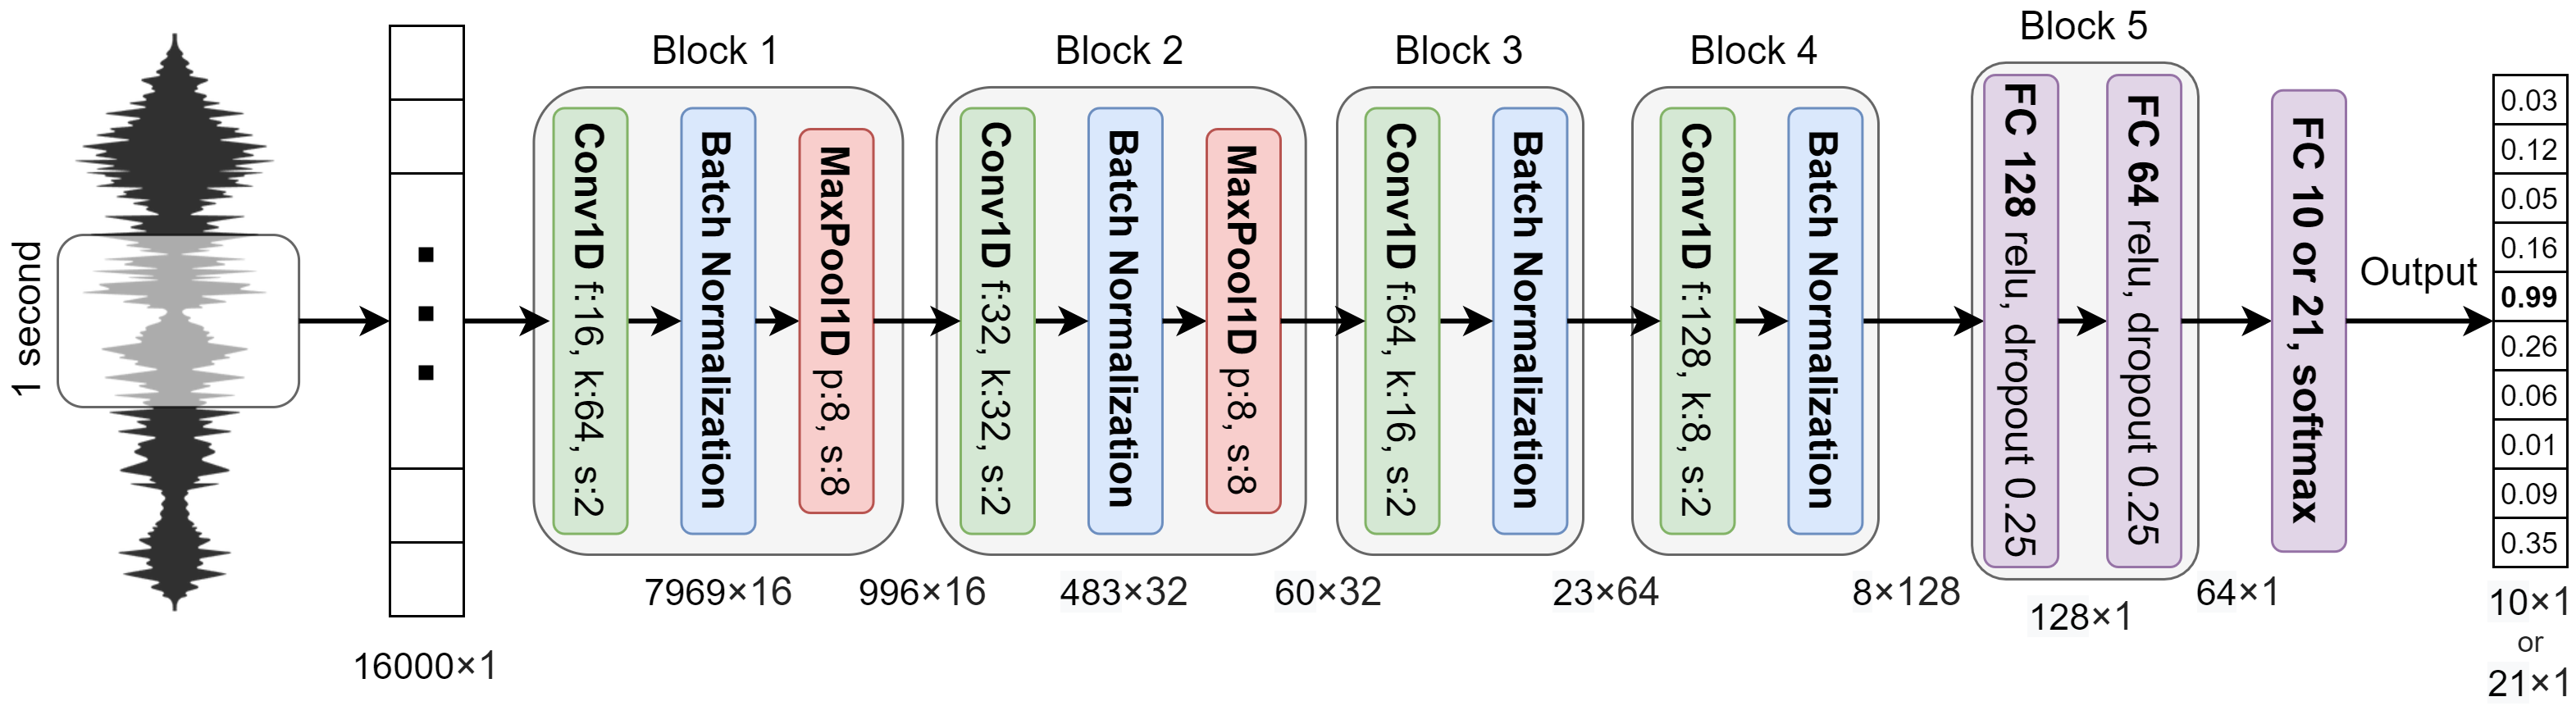
\includegraphics[scale=0.16]{1DCNN}

\begin{small}\textit{\textbf{Figure 2}: MANCA DESCRIZIONE}
\end{small}
\end{figure*}

The proposed architecture (shown in \textbf{\textit{Figure 2}}) is made of four \textit{convolutional layers} interlaced with max pooling layers and followed by two \textit{fully connected layers} and an output layer.

The input consists of an array of 16000 dimensions, which represents a 1-second audio sample at 16kHz.
The proposed 1D CNN has large receptive fields in the first convolutional layers since it is assumed that the first layers should have a more “global view” of the audio signal. The output of the last pooling layer for all feature maps is flattened and represents the input for a fully connected layer. In order to reduce overfitting, batch normalization is applied after the activation function of each convolution layer. After the last pooling layer, there are two fully connected layers with 128 and 64 neurons respectively; drop-out is applied with a probability of 0.25 for both layers.

Keeping in mind the architecture shown in \textbf{\textit{Figure 2}}, it is possible to omit a signal processing module because the network is strong enough to extract relevant low-level and high-level information from the audio waveform.

In the case of multiclass classification, the number of neurons of the output layer is the number of classes. Using the \textit{softmax} as activation function for the output layer, each output neuron indicates the membership degree of the input samples for each class.


%\newpage
\subsection{DSConv Model}
\begin{figure*}[t]
\centering
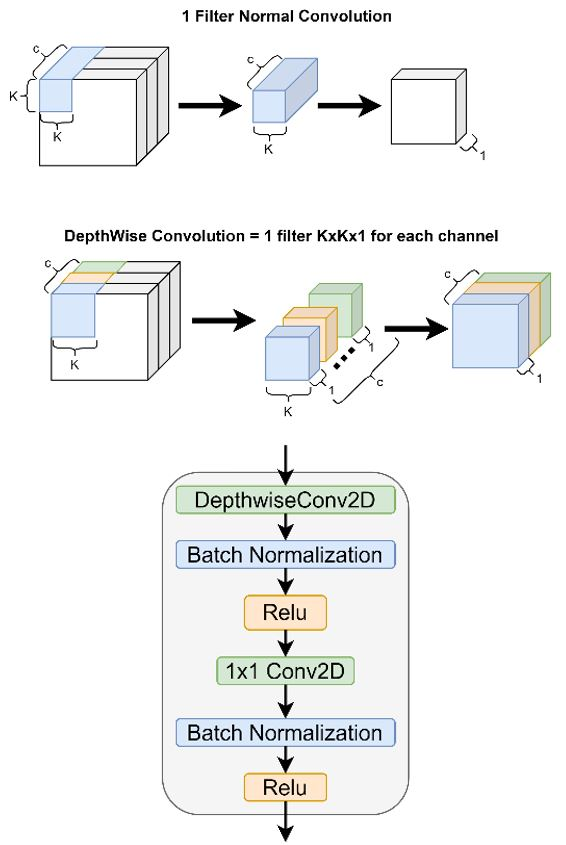
\includegraphics[scale=0.6]{confronto}

\begin{small}\textit{\textbf{Figure 3}: MANCA DESCRIZIONE}
\end{small}
\end{figure*}

This model uses \textit{Depthwise Separable Convolutions}. A separable convolution uses less parameters, less memory and less computations than regular convolutional layers, and in general it even perform better.

There are two types of Separable convolution: Spatial and Depthwise.
Spatial Separable Convolutions divide a kernel into two smaller kernels (e.g. division of a 3$\times$3 kernel into a 3$\times$1 and 1$\times$3 kernel). Instead of considering one convolution with 9 multiplications, we handled two convolutions with 3 multiplications each (6 in total) to achieve the same result. With a lower number of multiplications, the computational complexity significantly decreases, and the network is able to run and train faster.

Depthwise Separable Convolutions use kernels that cannot be “split” into two smaller kernels that do two convolutions: the \textit{depthwise convolution}, which result will be the input for the \textit{pointwise} (1$\times$1) one.

In \textbf{\textit{Figure 3}} you can see the difference between a normal 3D Convolution and a Depthwise, and the final Depthwise Separable Convolutions block we used. 



In our work we adopted a depthwise separable CNN inspired by the implementation of Hello Edge: Keyword Spotting on Microcontrollers.
This CNN is composed of a 2D CNN followed by batch normalization and 4 or 5 DSConv2D layers. An average pooling, with padding 2x2 and stride 2x2, followed by a fully-connected layer is used at the end to provide global interaction and reduce the total number of parameters in the final layer.
We implemented three different variants: large, medium and small, described in Table X, where we tried to reduce the number of parameters while maintaining a good accuracy.

\newpage
\subsection{Ensemble}
The ensemble simply took the two best models and did the average of their final prediction: in this way we reached the best accuracy, but at the cost of having a large network.

All models are trained with \textbf{Google Tensorflow 2.1} framework with \textbf{Keras} using the standard \textit{Sparse categorical cross entropy} and \textit{Nadam optimizer}. With a batch size of 32, the models were trained for 100 epochs with initial learning rate of $10^{-4}$. An early stopping with a patience of 10 epochs is applied to avoid overfitting.

\section{Results}
We trained each DSConv networks for all the features we described in Section IV to see if there were any differences between each set. As stated before, we used two different datasets, one made of ten class and another one of twenty-one.
We found that the number of convolutional layers played a key role in detecting high-level concepts both for DSconv model and 1DCNN model. The number of convolutional layers in our models was determined in an experiment using the audio files of the Google Speech Commands V2 dataset.
We faced the overfitting problem, recognizing the importance of the early-stopping procedure during the training comparing the test scores of the last epochs of the models with the best ones found by the ModelChekpoint function of Keras (using the validation set).
It took some time, for us, to choose the best metrics to be used to evaluate our models, and at the end we decided accuracy was the best choice. Due to the fact that in a problem where there is a large class imbalance, a model can predict the value of the majority class for all predictions and achieve a high classification accuracy. So, further performance measures are needed such as F1 score and Brier score, but since in our dataset classes are balanced, we can still use Accuracy. (DA RIGUARDARE)

We also measured the prediction speed of each model with and without Feature Extraction. We should not consider Multiplication as metrics because it is an indirect alternative for a direct metric such as latency.
Furthermore, we noticed that predicting one example or a batch made of ten examples requires the same amount of time, this happens because TensorFlow make tensors operations. In the final implementation this fact should be taken into account in order to minimize the computational cost.
In tables X,Y,Z,W,P you can see the accuracy and the speed prediction of our models.
The most performant ones are …
As you can see using 40MFCCs + deltas does not perform better, on the contrary the models have worse accuracy, a larger number of parameters and they are slower.
There is no much difference between using 80 Mels or 40 MFCCs, calculating MFCC requires slightly more time since they are calculated after the Mels but MFCC requires almost the half of parameters.
The fastest network is the 1D CNN on RAW data since it has not to calculate any feature extraction, but is the worst in terms of accuracy.
The best accuracy is obtained by the ensemble network, but it is obviously the slower and the bigger model.
The smallest model is the DSConvSmall + 40MFCCs with 127K parameters, 92.9% accuracy and 38.23 ms of prediction speed.


\section{Concluding Remarks}
In this paper, an end-to-end architecture for the keyword spotting task has been proposed. We built two neural networks and an ensemble between the best models.
The 1D CNN consists of five convolutional layers. Instead of using handcrafted static filterbanks (such as the ones used to extract MFCC features), the proposed 1D CNN learns the filters directly from the audio waveform. The other network receives as input features 80Mels, 40MFCCs or 40MFCCs+deltas and consists of 4 or 5 DSConv layers.
Furthermore, the 1D CNN is faster than the other models, but unfortunately does not reach the same accuracy.
As we can see from the results we obtained, all the features work well but 40MFCCs seems slightly better that the others and the 1DCNN on RAW waveform was the worst.
We further reduce the number of parameters of the DSConv model by reducing the number of the filters for each convolution. We proposed three version of the DSConv model: Large, medium and small.
Our models achieve excellent results but we did not beat the state of the art accuracy of 97.4% reached by SMALL-FOOTPRINT KEYWORD SPOTTING ON RAW AUDIO DATA WITH SINC-CONVOLUTIONS. You can find a summary of our model compared with the state of the art in TABLE X.
We noticed that if we pick more frames per second as described in the end-to-end architecture the model has many “point of view” of the word, so in the real world it actually performs better than the test accuracy measured. In various tests we made, also the 1D CNN, that is the one with the worse accuracy, captured all the words we were saying thanks to the multiple windows – fusion rule technique.

Further improvement could be exploring the SincConv,….

You can find the code on github [X]

[WHAT WE LEARNT AS STUDENTS]


\section*{Acknowledgment}
All the experiments were conducted using Keras and blabla libraries.

The authors would like to acknowledge the support of...


\begin{thebibliography}{1}
\bibitem{1}
Douglas Coimbra de Andrade, Sabato Leo, Martin Loesener Da Silva Viana, Christoph Bernkopf. \textit{A neural attention model for speech command recognition}. arXiv:1808.08929

\bibitem{2}
Jan Chorowski, Dzmitry Bahdanau, Dmitriy Serdyuk, Kyunghyun Cho, Yoshua Bengio. \textit{Attention-Based Models for Speech Recognition}. arXiv:1506.07503

\bibitem{3}
Sainath, Tara N. / Parada, Carolina (2015). \textit{Convolutional neural networks for small-footprint keyword spotting}, In INTERSPEECH-2015, 1478-1482.

\bibitem{4}
Raphael Tang, Jimmy Lin. \textit{Deep Residual Learning for Small-Footprint Keyword Spotting}. arXiv:1710.10361

\bibitem{5}
Alon, G.. \textit{Key-Word Spotting-The Base Technology for Speech Analytics}.

\bibitem{6}
Pete Warden. \textit{Speech Commands: A Dataset for Limited-Vocabulary Speech Recognition}.
\end{thebibliography}
\end{document}


